\documentclass[a4paper]{article}

\usepackage[utf8]{inputenc}
\usepackage[french]{babel}
\usepackage{fullpage}

\usepackage{amsmath}
\usepackage{amssymb}
\usepackage{latexsym}

\usepackage{listings}
\lstloadlanguages{Haskell}
\usepackage{minitoc}
\usepackage{ifpdf}

\ifpdf
\usepackage[pdftex]{graphicx}
\else
\usepackage{graphicx}
\fi

\title{PuissanceHask}
\author{Adrien DUDOUIT-EXPOSITO\\Alexandre LEGOUPIL}

\date{2012-01-23}

\begin{document}

\ifpdf
\DeclareGraphicsExtensions{.pdf, .jpg, .png}
\else
\DeclareGraphicsExtensions{.eps, .jpg}
\fi

\maketitle


\begin{abstract}
PuissanceHask est une implémentation en Haskell du jeu de Puissance 4.
\end{abstract}
\section*{Introduction}
Nous avons créer une version jouable et parfaitement fonctionnelle du jeu puissance 4 en haskell celui ci dispose d'une interface textuelle. Permettant de jouer agréablement et avec une certaine protection contre les erreurs de la part du joueur.  
\newpage
\section{Structure du programme}

Pour le programme il a été choisi une architecture de module où chaque fonction telle que l'IA, les structure, les règles de jeux, les mécanismes de jeu, et l'interface son chacun dans un module et le programme principale n'appel que le main défini dans l'interface, l'interface appel les structures et les mécanismes de jeu qui eux appel leqs règles. Ainsi il est possible de changer de type d'IA ou d'interface en une unique ligne.

\section{Intelligence Artificielle}

Pour l'intelligence artificiel un algorithme MiniMax a été utilisé. D'autres méthode de choix de coups on été implémenté moins couteuse on été implémenté pour pouvoir tester plus facilement comme un algorithme qui remplit toujours la première colonne disponible ou encore un algorithme qui remplit toujours la ligne la moins remplie.

\subsection{Algorithme MiniMax}
\label{alg:minimax}

Wikipédia nous donne la définition suivante:
\begin{quote}
L'algorithme minimax est un algorithme qui s'applique à la théorie des jeux pour les jeux à deux joueurs à somme nulle. Pour une vaste famille de jeux, le théorème du minimax de von Neumann assure l'existence d'un tel algorithme, même si dans la pratique il n'est souvent guère aisé de le trouver. Le jeu de hex est un exemple où l'existence d'un tel algorithme est établie et montre que le premier joueur peut toujours gagner, sans pour autant que cette stratégie soit connue.

Il amène l'ordinateur à passer en revue toutes les possibilités pour un nombre limité de coups et à leur assigner une valeur qui prend en compte les bénéfices pour le joueur et pour son adversaire. Le meilleur choix est alors celui qui minimise les pertes du joueur tout en supposant que l'adversaire cherche au contraire à les maximiser (le jeu est à somme nulle).
\end{quote}

Ainsi on construit d'abord un arbre de possibilité, où un n\oe ud ou une feuille représente un coups et est valué. De plus chaque n\oe ud possède un nombre de fils inférieur ou égal au nombre de colonnes dans le jeu.

Pour généré un arbre de possible on envisage chaque placement sur chaque colonne et on évalue chaque coup selon la méthode suivante:

\begin{lstlisting}
si le coup n'est pas gagnant
vaut -10
si le coup est gagnant pour le joueur
vaut 100
si le coup est perdant pour le joueur
vaut -100
\end{lstlisting}

Lors de l'implémentation l'évaluation est simultané avec la construction de l'arbre:

\begin{lstlisting}[language=haskell]
nextMMTree :: Int -> Table -> Token -> (Int,Token) -> MMTree
nextMMTree diff table token (p,t)
| not (isFreeCol table p) = MMLeaf (p,t) 0
| sameToken win ( Just token ) = MMLeaf (p,t) winVal
| isJust win = MMLeaf (p,t) looVal
| diff == 0 = MMLeaf (p,t) blankVal
| otherwise = MMNode (p,t) blankVal ( constructMMTree (diff-1)
next token )
where
next = placeToken table p t
win = gameWinner next
winVal = 100
looVal = (-100)
blankVal = (-10)
\end{lstlisting}

Un fois l'arbre construit on applique a chaque n\oe ud le traitement suivant:

\begin{lstlisting}
si p est une feuille
minimax(p) = evaluer(p)
si p est un noeud Joueur avec fils O1, ..., On
minimax(p) = evaluer(p) + MAX(minimax(O1), ..., minimax(On))
si p est un noeud Opposant avec fils O1, ..., On
minimax(p) = evaluer(p) + MIN(minimax(O1), ..., minimax(On))
\end{lstlisting}

Implémenté ainsi:

\begin{lstlisting}[language=haskell]
computeMMTree :: Token -> MMTree -> (Maybe Int,Int)
computeMMTree token (MMNode (a, t) v c)
| token == t = (\(_,x) -> (Just a, v+x)) . bestCoin $
map ( computeMMTree token ) c
| otherwise = (\(_,x) -> (Just a, v+x)) . worstCoin $
map ( computeMMTree token ) c
computeMMTree _ (MMLeaf (a, _) v) = (Just a, v)
\end{lstlisting}

Où les fonction $bestCoin$ et $worstCoin$ sélectionnent respectivement le meilleur ou moins bon coup a jouer pour le joueur ($worstCoin$ sélectionne le meilleur coup adverse).
\subsection{Performances}

Comme présenté sur le graphique  la complexité exponentielle à un coup en temps assez élever se qui ne permet pas de faire des arbres de profondeur supérieur a 5.

\begin{figure}[h!]
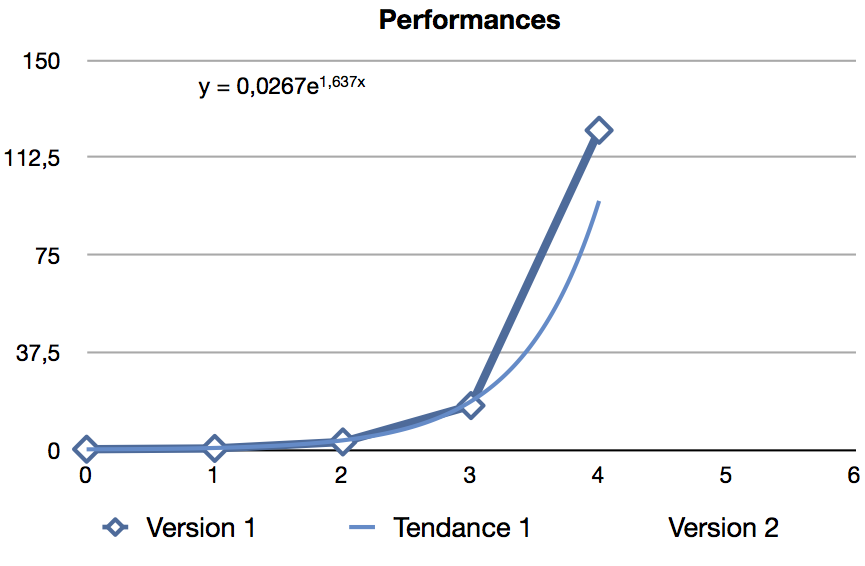
\includegraphics[scale=0.88]{Performance}
\end{figure}

\subsection{Optimisation}

Les principale source de calcul sont d'une part la création de l'arbre mais aussi et surtout le choix du meilleur élément qui peut être exécuté jusqu'à 79 000 fois lors d'un un appel (cas d'une recherche jusqu'à 6 coups en avance)
\newpage
\section{Solutions choisies}	%fold
Le plateau pour des raisons pratique est un carré de 7 par 7 .Cette dimension est modifiable dans le fichier data on peut ainsi jouer sur un plateau de 100 par 100 sans soucis.\\
L'interface du jeux est la fenêtre shell du compilateur se qui ce révèle être un inconvénient au point de vue esthétique mais permet au final une plus grande portabilité du jeux en n'obligeant pas l'utilisateur à installer une librairie graphique spécifique.\\
L'interface est relativement bien protégé contre les erreur volontaire ou non de l'utilisateur.

% section Solutions choisies(end)

\section{Problèmes rencontrés}	%fold
Au début le programme devait être doté d'une interface graphique grâce à des libraires tel que hOpenGL ou WXhaskell, toutefois nous avons été dans l'incapacité d'installer ces librairies : hOpenGL est rarement mis à jour, son installation est nébuleuse et ses tutoriel sont dépassé.\\
WXhaskell quand à lui dispose de plus de mise à jour mais malgré différents essais (sur windows et linux) nous avons été incapable de la rendre opérationnel.\\
Nous nous somme donc rabattu sur une interface shell certes moins esthétique mais totalement fonctionnel.Même si un premier jet de l'interface en wxhaskel à été crée\footnote{voir Annexe}.

% section Problèmes rencontrés(end)

\section{Détails du jeux}
\begin{itemize}
\item Les colonnes sont numérotés de 1 à 8 dans la configuration de base.
\item Le plateau est un carré de 7 par 7 dans la configuration de base.
\item Le joueur humain joue avec les croix et l'IA avec les rond.
\item Le joueur commencera toujours la partie.
\end{itemize}
% section Détails du jeux(end)
\subsection{Régles du jeux}
Le gagnant est celui qui le premier réussira a aligner sur une colonne ligne ou diagonal 4 de ses pions, si le plateau est remplis sans qu'il y ait un gagnant la partie se conclue  par un match nul.
\newpage
\section{mode d'emploi} %fold
Pour utiliser le jeu compilez le fichier puissanceHask et taper la commande main : le jeu est lancé .\\
Les réglés du jeu vous sont expliquées puis une nouvelle partie est lancé avec l'affichage du plateau et l'on vous demande de donner un numéro de colonne ou placer votre jeton ( exemple-ci dessous).

\begin{figure}[!h] %on ouvre l'environnement figure
	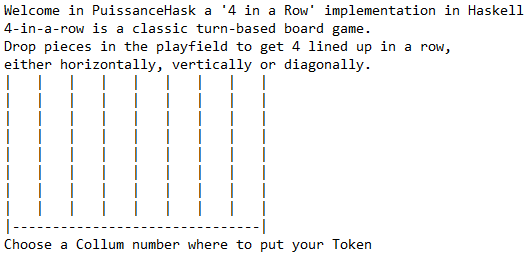
\includegraphics[width=14cm]{lancement}
		\caption{Le jeu au lancement}
	\end{figure}

Ensuite vous devez attendre que le programme affiche votre coup et celui de l'ordinateur sur le plateau,\\
puis on vous redemandera de donner le numéro d'une colonne( exemple-ci dessous).\\

\begin{figure}[!h] %on ouvre l'environnement figure
	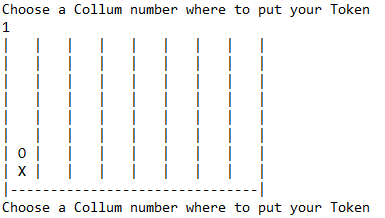
\includegraphics[width=10cm]{coup}
		\caption{aprés quelques coups}
	\end{figure}

Et ainsi de suite jusqu'à la défaite de l'humain, de l'ordinateur ou du match nul.\\
Une fois la partie terminé il vous sera demandé si vous voulez rejouer si vous refusez vous quitterez le jeu. 

Toute utilisation d'un caractère autre qu'un numéro entrainera la fin de la partie. Les numéros irrecevable ne seront pas pris en compte et une nouvelle chance vous serra donnée. 
% section mode d'emploi(end)

\newpage
\section{Annexe} %fold
\subsection*{Debut d'une interface utilisant wxHaskell}
\lstinputlisting{wxMain.hs}

% section Annexe(end)
\bibliographystyle{plain}
\bibliography{}
\end{document}
